\documentclass[11pt,UTF8]{report}

\usepackage{ctex}

\usepackage{listings}
\usepackage{xcolor}

\usepackage{graphicx}

\lstset{
    basicstyle=\tt,
    %行号
%    numbers=left,
%    rulesepcolor=\color{red!20!green!20!blue!20},
%    escapeinside=``,
%    xleftmargin=2em,xrightmargin=2em, aboveskip=1em,
    %背景框
%    framexleftmargin=1.5mm,
%    frame=shadowbox,
    %背景色
%    backgroundcolor=\color[RGB]{245,245,244},
    %样式
    keywordstyle=\color{blue}\bfseries,
    identifierstyle=\bf,
    numberstyle=\color[RGB]{0,192,192},
    commentstyle=\it\color[RGB]{96,96,96},
    stringstyle=\rmfamily\slshape\color[RGB]{128,0,0},
    %显示空格
    showstringspaces=false
}

\renewcommand\thesection{\arabic{section}}

\title{数据库系统概论大作业报告}
\author{杜政晓 2016011014\\
吴一凡 }
\begin{document}
\maketitle

\section{系统功能}

\section{系统架构设计}
\begin{figure}[!ht]
	\centering
	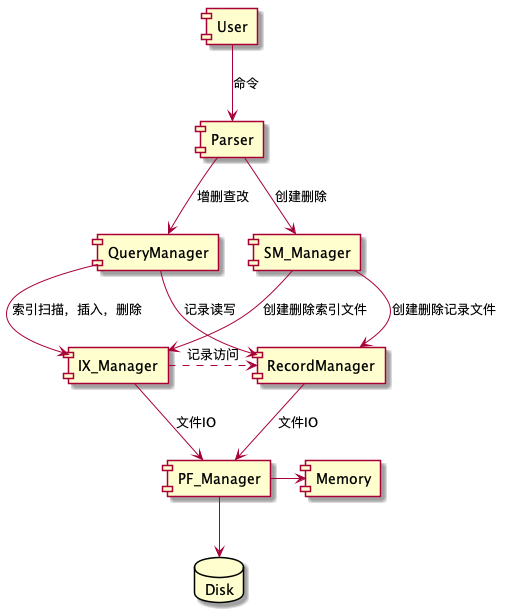
\includegraphics[width=0.9\textwidth]{structure}
\end{figure}
\section{各模块详细设计}
\subsection{记录管理模块}
\subsubsection{文件结构设计:}
每个文件只存储同一类长度相等的记录。文件由页(Page)组成,,页由大小等于记录长度的槽(Slot)组成。
每个文件的第一页作为文件头,保存了文件的一些元信息,比如记录长度、文件中的页数目、文件中的记录数目等。
文件中每一页的开头保存了该页的一些基本信息。比如该页的槽哪些是空的哪些是非空的。这里使用了Bitmap来表示槽的空与非空。此外,为了能够在插入记录的时候能够快速找到有空槽的页,使用了一个链表来存储有空槽的页。首页中保存了链表中的第一项的页码。每一页的开头4个字节指向的是链表中下一项的页码。比起在首页中用Bitmap来表示页是否非空,这种方式能够存储的页数是没有限制的。

\subsubsection{模块具体实现}

因为在使用提供的页式文件管理系统的时候出现了奇怪的bug(具体表现是缓存的hash表有时候会突然“丢掉”某个已经打开的页,导致该页对应的页数变成了一个随机数)。而且该文件系统的功能不全(比如没有将某个页固定在缓存中不要换出的功能,在关闭文件的时候也不会写回它的所有页),所以我换用了CS346中提供的页式文件管理系统。
RecordManager的创建、删除文件都使用文件管理系统的接口。打开文件除了调用接口外,还会将文件的首页中的信息复制出来,并设置modified为false。如果后续操作中改变了首页信息则将modified设置为true。当关闭文件的时候,如果发现modified为true,则将复制出来的信息写回文件的首页。
RM\_FileHandle负责对文件中的记录进行管理。插入记录时,从首页中找到有空槽的页,然后进行插入。如果发现插入之后该页已经满了,则将首页上有空槽的页码换为链表中的下一项。在删除记录的时候,只需要将Bitmap的对应位设置为空,然后将该页的页码插入到链表的开头。
对文件的扫描由RM\_FileScan进行,其方法就是依次遍历每一页,每一页中遍历Bitmap中的每一个非空位对应的槽。

\section{主要接口说明}
\subsection{记录管理模块}
记录管理模块的核心是类RecordManager,用于实现记录管理中文件级别的操作,其接口包括:
\begin{lstlisting}[language=C++]
// Create a file with filename and record size
int createFile (std::string filename, unsigned record_size);
// Delete a file with filename
int destroyFile(std::string filename);
// Open a file with filename in file_handle
int openFile(std::string filename, RM_FileHandle &file_handle);
// Close the file opened in file_handle
int closeFile(RM_FileHandle &file_handle);
​\end{lstlisting}

通过RecordManager打开的文件会返回一个RM\_FileHandle,用于实现对于单个文件中记录的操作
\begin{lstlisting}[language=C++]
// Get a record by rid
int getRec(const RID &rid, RM_Record & record) const;
// Insert a new record and return the rid
RID insertRec(const char *pData);
// Delete a record by rid
int deleteRec(const RID &rid);
// Update a record
int updateRec(const RM_Record &rec);
\end{lstlisting}

此外还有一个类RM\_FileScan用来进行对文件中记录的查询
\begin{lstlisting}[language=C++]
// Initialize file scan
int openScan(const RM_FileHandle &fileHandle,
             AttrType attrType,
             int attrLength,
             int attrOffset,
             CompOp compOp,
             void *value
);
// Get next matching record
int getNextRec(RM_Record &rec);
// Terminate file scan
int closeScan();
\end{lstlisting}

注意在记录管理模块中我们只实现了对记录中单个属性值进行限制的查询。

\section{实验结果}

\section{小组分工}
\begin{itemize}
	\item 杜政晓:记录管理模块,查询处理模块,SQL parser
	\item 吴一凡:索引管理模块,系统管理模块
\end{itemize}

\section{参考文献}
\end{document}
